\documentclass[french,english,12pt]{article}
\usepackage[utf8]{inputenc}
\usepackage[T1]{fontenc}
\usepackage{lmodern}
\usepackage[a4paper]{geometry}
\usepackage{babel}
\usepackage{xcolor}   
\usepackage{amsmath}
\usepackage{booktabs}
\usepackage{amsfonts}
\usepackage{amssymb}
\usepackage{graphicx}
\usepackage{listings}
\usepackage{color}
\usepackage{url}
\usepackage{float}
\restylefloat{table}
\usepackage{textcomp}
\usepackage{pgfplots,pgfplotstable}
\usepackage{tikz}
\usetikzlibrary{arrows,backgrounds,mindmap,positioning,shadows,shapes}
\definecolor{listinggray}{gray}{0.9}
\definecolor{lbcolor}{rgb}{0.9,0.9,0.9}

\pgfplotstableset{
every head row/.style={before row=\toprule,after row=\midrule},
every last row/.style={after row=\bottomrule}}


\lstset{
	backgroundcolor=\color{lbcolor},
	tabsize=4,
	rulecolor=,
	language=C++,
        basicstyle=\scriptsize,
        upquote=true,
        aboveskip={1.5\baselineskip},
        columns=fixed,
        showstringspaces=false,
        extendedchars=true,
        breaklines=true,
        prebreak = \raisebox{0ex}[0ex][0ex]{\ensuremath{\hookleftarrow}},
        frame=single,
        showtabs=false,
        showspaces=false,
        showstringspaces=false,
        identifierstyle=\ttfamily,
        keywordstyle=\color[rgb]{0,0,1},
        commentstyle=\it\tt\color[rgb]{0.133,0.545,0.133},
        stringstyle=\color[rgb]{0.627,0.126,0.941},
        inputencoding=utf8
        }

\lstset{escapeinside={(*@}{@*)}}
\lstset{includerangemarker=false,rangeprefix=\/\/\#\ ,% curly left brace plus space
  rangesuffix=\ \#}% space plus curly right brace



\begin{document}
\begin{titlepage}
\begin{center}
  \Huge
  \textbf{UFR de Mathématiques et d'Informatique de Strasbourg}
  \par \vspace{2 cm}
  \textbf{Projet Éléments finis}
  \par \vspace{1 cm}
  \emph{M2 CSMI}
  \par \vspace{5 cm}
  \bsc{Lantz} Thomas
  \par \vspace{3 cm}
  \normalsize{\today}\\
  \end{center}
\end{titlepage}

\newpage
\tableofcontents
\newpage

\section{An Agile software development method : Extreme programming }

First at all,we will start to explain what Agile development is about. It's a group of several software development methods bases on iterative development,in other words with quick release, and on a huge interest on feedback from differents sources.\\
We will interest us here about one of this methods, known as the Extreme programming (or XP method).\\

\subsection{Concept}

Extreme programming take his name in the fact that all the normal code practices are pushed to an extreme limit. Like we said before, Extreme programming take place in Agile software developement methods. In this way, it follow the bases of them, with the iterative development and feedback importance. At this, we can include also some specificities like pair programming or "simplicity" coding for example.

\subsubsection{Iterative development and Feedback}

Iterative development is one of the most important features in the Agile software development. We choose to shorten the release time between each new code. This will result in smaller code portion but in a larger ammount than normal coding style. This is particuliary useful to check that we are not going in the wrong way, or to change it if the customer want to modify the original project. Futhermore, this feature will complete well the others, that will be presented next.\\

Here is an iterative diagram for the Extreme programming method :\\

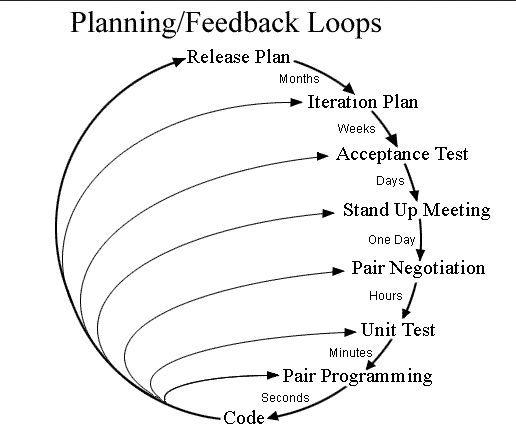
\includegraphics[scale=0.40]{Extrem_Diagram.png} 

Source : \url{http://en.wikipedia.org/wiki/Extreme_programming}

In fact, Iterative method work well with the idea of important feedback. Feedback can be obtain from differents sources,like :\\
\begin{itemize}
\item System feedback, with code testing for example.
\item Customer feedback, with regular talk.
\item Team feedback, with pair programming.
\end{itemize}

The fact that we build code with short release, we have system feedback frenquently with code test, and the correction, if necessary, can be made quickly.

\subsection{Pair Programming and "Simplicity" Coding}

Pair programming, as it's name suggests, is a technique where two programmer work together on the same programm.
One of them write the code, as the other check and review the code lines.\\

They are some benefits to used this technique:
\begin{itemize}
\item  Like we talk about before, it's a form of feedback used by Agile software development.
\item Each participant can focus on one part of the code at the time, that increase the result.
\item Communication between the two programmers enable to increase the programming level.
\end{itemize}
\vspace{1 cm}
As for the "simplcity" coding, it's a sort of point of view adopted by Extreme programming coders. It can be explain by the following setence : " Code what you need now, and not what you will need in the future ".
As before, the fact that the code is build litle by litle, with a sort time between each release, is good complement to this vision. 

\section{Conclusion}

In conclusion, the Extreme programming method is a technique, that consist in cuting the software development into smaller but regular releases, with an important place of feedback during the projet path.\\

It's a different coding method that I used to know, but it seems pretty useful for big projet, with team construction.

\end{document}

